%==============================================================
%  Position Bias: Estimation and Correction
%==============================================================
\chapter{Position Bias: Estimation and Correction}
\label{ch:position-bias}

The recommendations served on IndiaMART are consumed as ranked lists, and the
rank at which an item appears strongly shapes whether a user interacts with it.
Items placed near the top are seen and clicked far more often than items placed
lower, irrespective of their true relevance. Learning a recommender directly
from such click logs therefore bakes in the artefacts of presentation: the
model is rewarded for what was \emph{shown prominently}, not for what was
\emph{actually relevant}. This chapter is concerned with making that distortion
explicit --- modelling it, estimating it from data, and correcting for it ---
and with feeding the correction back into the recommendation engine.

The recommendation engine itself, a $K$-step graph-diffusion model, is not a
contribution of this work; it pre-existed and is summarised here only to the
extent needed to explain where the bias correction is applied
(Section~\ref{sec:pb-kstep}). The contribution is the estimation of position
bias and its integration as transition weights. The dataset on which all of
this rests is described in its own chapter; here we refer to its fields only as
needed.

%--------------------------------------------------------------
\section{The Position-Bias Problem}
\label{sec:pb-problem}

Top-ranked results enjoy higher visibility, and users interact more with
higher-listed items simply because they are higher-listed. The consequence is
twofold. First, \emph{learning} is unfair: a model trained on raw clicks
confuses prominence with relevance and perpetuates whatever ordering was
historically shown. Second, \emph{evaluation} is inaccurate: a click-through
metric computed on biased exposure rewards a system for exploiting position
rather than for surfacing genuinely useful items. If position bias is left
uncorrected, both the learning signal and the yardstick used to judge it are
compromised. The central challenge addressed here is thus to \emph{estimate}
the position bias and to \emph{correct} for it, so that the recommender learns
from a relevance signal rather than an exposure signal.

The effect is visible directly in the click logs. Figure~\ref{fig:pb-clicks}
shows the total number of clicks as a function of the rank at which the clicked
item was shown: clicks fall monotonically from the first position downward, a
canonical signature of position bias.

\begin{figure}[ht]
  \centering
  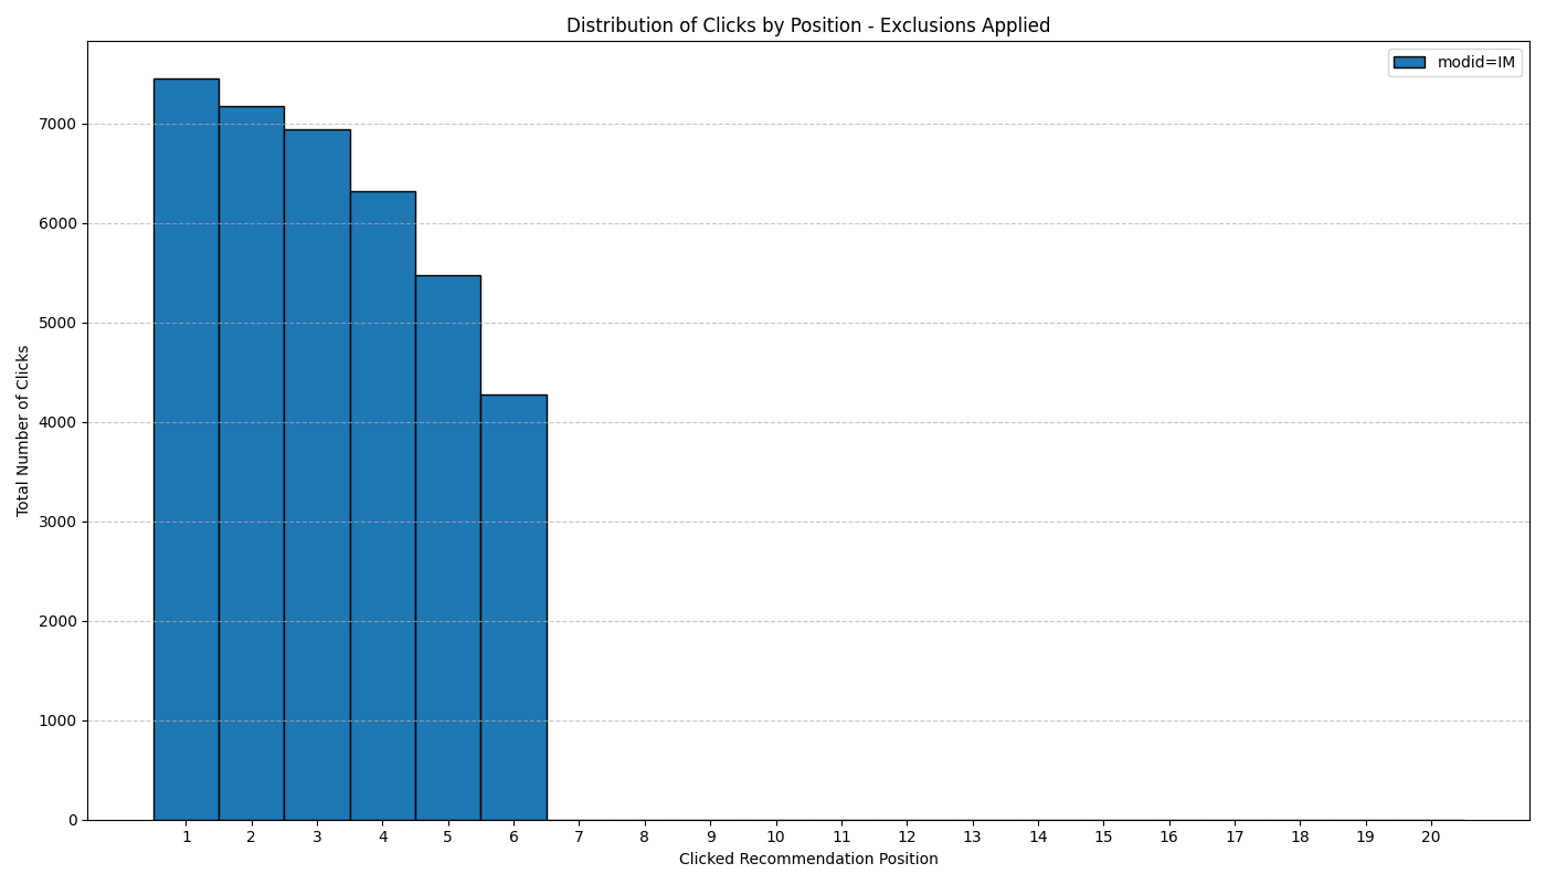
\includegraphics[width=0.85\textwidth]{figures/position-clicks.png}
  \caption{Observed clicks by position. The monotone decline with rank is
           direct evidence of position bias.}
  \label{fig:pb-clicks}
\end{figure}

%--------------------------------------------------------------
\section{A Click Model for Position Bias}
\label{sec:pb-model}

We adopt the \emph{examination hypothesis}~\cite{Craswell08}, the standard
factorisation underlying position-bias work. It posits that a click occurs only
when the user both \emph{examines} the item's slot and finds the item
\emph{relevant}, and that these two events are independent:
\begin{equation}
  \label{eq:exam}
  P(C{=}1 \mid i,j,k)
    \;=\; P(E{=}1 \mid k)\,\cdot\,P(R{=}1 \mid i,j)
    \;=\; \pi_k \,\cdot\, P(R{=}1 \mid i,j).
\end{equation}
Here $C$ is the observed click ($C{=}1$ for a click), $E$ the examination
event, and $R$ the relevance event. The factor $P(E{=}1\mid k)=\pi_k$ is the
\emph{position bias} at rank $k$ --- the probability that a user examines the
slot at rank $k$, depending on the rank alone. The factor
$P(R{=}1\mid i,j)$ is the true relevance of item $i$ given the context item
$j$, independent of where $i$ is shown.

At the level of counts, let $n_{i,j,k}$ be the number of observed clicks on
item $i$ when it is shown at position $k$ in the list for context $j$, and let
$n_j$ be the number of exposures of context $j$. Writing $P(i\mid j)$ for the
relevance of $i$ given $j$, the expected click count is
\begin{equation}
  \label{eq:expected}
  \mathbb{E}\!\left[n_{i,j,k}\right]
    \;=\; n_j \,\cdot\, P(i\mid j) \,\cdot\, \pi_k .
\end{equation}
Equation~\eqref{eq:expected} is the count-level form of
\eqref{eq:exam} and is the workhorse of the estimation that follows: every
observed click count is the product of an exposure term ($n_j$), a
position-independent relevance term ($P(i\mid j)$), and a relevance-independent
position term ($\pi_k$). Estimating $\pi_k$ amounts to isolating the last
factor from the other two.

%--------------------------------------------------------------
\section{Estimating Position Bias}
\label{sec:pb-estimate}

Three complementary routes to $\pi_k$ were pursued: a direct aggregation under
a perfect-exposure assumption, an anchoring of the bias to external traffic
sources, and a controlled A/B estimation.

\subsection{Perfect-Exposure Aggregation}
\label{sec:pb-perfect}
If a position is filled by a sufficiently wide variety of items across many
contexts --- as in a large search system --- then aggregating clicks over all
items and contexts at a fixed rank $k$ averages out the relevance term and
leaves the position term. Summing \eqref{eq:expected} over $i$ and $j$,
\begin{align}
  \sum_{i,j} n_{i,j,k}
    &= \sum_{i,j} n_j\,P(i\mid j)\,\pi_k
     = \pi_k \sum_{j} n_j \sum_{i} P(i\mid j),
  \label{eq:perfect-sum}
\end{align}
so that the position bias is recovered as
\begin{equation}
  \label{eq:perfect-pi}
  \pi_k \;=\;
    \frac{\sum_{i,j} n_{i,j,k}}
         {\sum_{j} n_j \sum_{i} P(i\mid j)} .
\end{equation}
This is the \emph{perfect-exposure} estimator: under the idealisation that all
positions see a comparable mix of items, the numerator is just the total clicks
at rank $k$ and the denominator is a normaliser shared across ranks, so the
$\pi_k$ are read off directly from rank-wise click totals.

\subsection{Anchoring to External Sources}
\label{sec:pb-external}
The second route treats \emph{other traffic sources} as if they were
additional positions, each with its own examination probability. In
particular, an external search engine such as Google can be regarded as a
``position'' with bias $\pi_g$, assumed independent of the on-platform ranks.
Applying \eqref{eq:expected} to the external source $g$ and to an on-platform
rank $k$ for the same context,
\begin{align}
  \mathbb{E}\!\left[n_{i,j,g}\right] &= n_j\,P(i\mid j)\,\pi_g, \label{eq:src-g}\\
  \mathbb{E}\!\left[n_{i,j,k}\right] &= n_j\,P(i\mid j)\,\pi_k. \label{eq:src-k}
\end{align}
Because the exposure and relevance terms are common to both, taking the ratio
of observed relevant clicks $c_i$ (at rank $i$) and $c_g$ (at the external
source) cancels them and exposes a pure bias ratio:
\begin{equation}
  \label{eq:ratio}
  \frac{\pi_i}{\pi_g} \;=\; \frac{c_i}{c_g}.
\end{equation}
Accumulating observed clicks at the various positions over historical data then
yields a ratio for every rank against the common anchor,
\begin{equation}
  \label{eq:hist-ratios}
  \frac{\pi_1}{\pi_g} = \frac{c_1}{c_g}, \qquad
  \frac{\pi_2}{\pi_g} = \frac{c_2}{c_g}, \qquad \dots
\end{equation}
so that all positions are placed on a common scale defined by the reference
source. Two reference sources were used in this way: Google search and
IndiaMART's own search. Because the raw view volumes from these search surfaces
are much smaller than the transition (recommendation) view volumes, the search
counts are \emph{scaled} to match the transition view volume before the ratios
are formed; the resulting curves are reported as ``adjusted'' quality ratios.

\subsection{A/B Estimation}
\label{sec:pb-ab}
The third route estimates bias by controlled experiment, which avoids relying
on the perfect-exposure idealisation. Users are split into two groups. Group A
is shown the recommendation list in its natural order; Group B is shown a
\emph{shifted} list, so that an item appearing at one rank for one group
appears at a different rank for the other. Let $n_A\!\big(\tfrac{p_2}{p_1},
k{=}2\big)$ be the clicks in Group A on the pair $p_1\!\to\!p_2$ at rank $2$,
and $n_B\!\big(\tfrac{p_2}{p_1}, k{=}1\big)$ the clicks in Group B on the same
pair at rank $1$. Since for either group
\begin{equation}
  \label{eq:ab}
  n\!\left(\tfrac{p_2}{p_1},\, k{=}i\right) \;\propto\; P(p_2\mid p_1)\,\pi_i,
\end{equation}
the shared relevance $P(p_2\mid p_1)$ cancels when the same pair is compared
across the two groups at the two ranks, leaving the bias ratio
$\pi_2/\pi_1$ directly. Showing the same item pair at swapped ranks to
statistically equivalent audiences is therefore a clean way to read off the
relative examination probabilities.

%--------------------------------------------------------------
\section{Empirical Findings}
\label{sec:pb-findings}

The estimators above were applied to roughly a year of logs (July~2024 through
May~2025), restricted in the diagnostic plots to the top $25\%$ of contexts by
volume so that the ratios are computed where data is densest.

\paragraph{Position 1 versus other positions.}
Figure~\ref{fig:pb-pos1} reports the weekly \emph{effectiveness ratio}
$\pi_1/\pi_i$ of the first position against each lower position. The ratios sit
broadly above unity and grow with rank distance --- position~5 in particular
spikes to between two and five times position~1 in many weeks --- confirming
that the first position attracts disproportionately more clicks than lower
ones for the same underlying relevance.

\begin{figure}[ht]
  \centering
  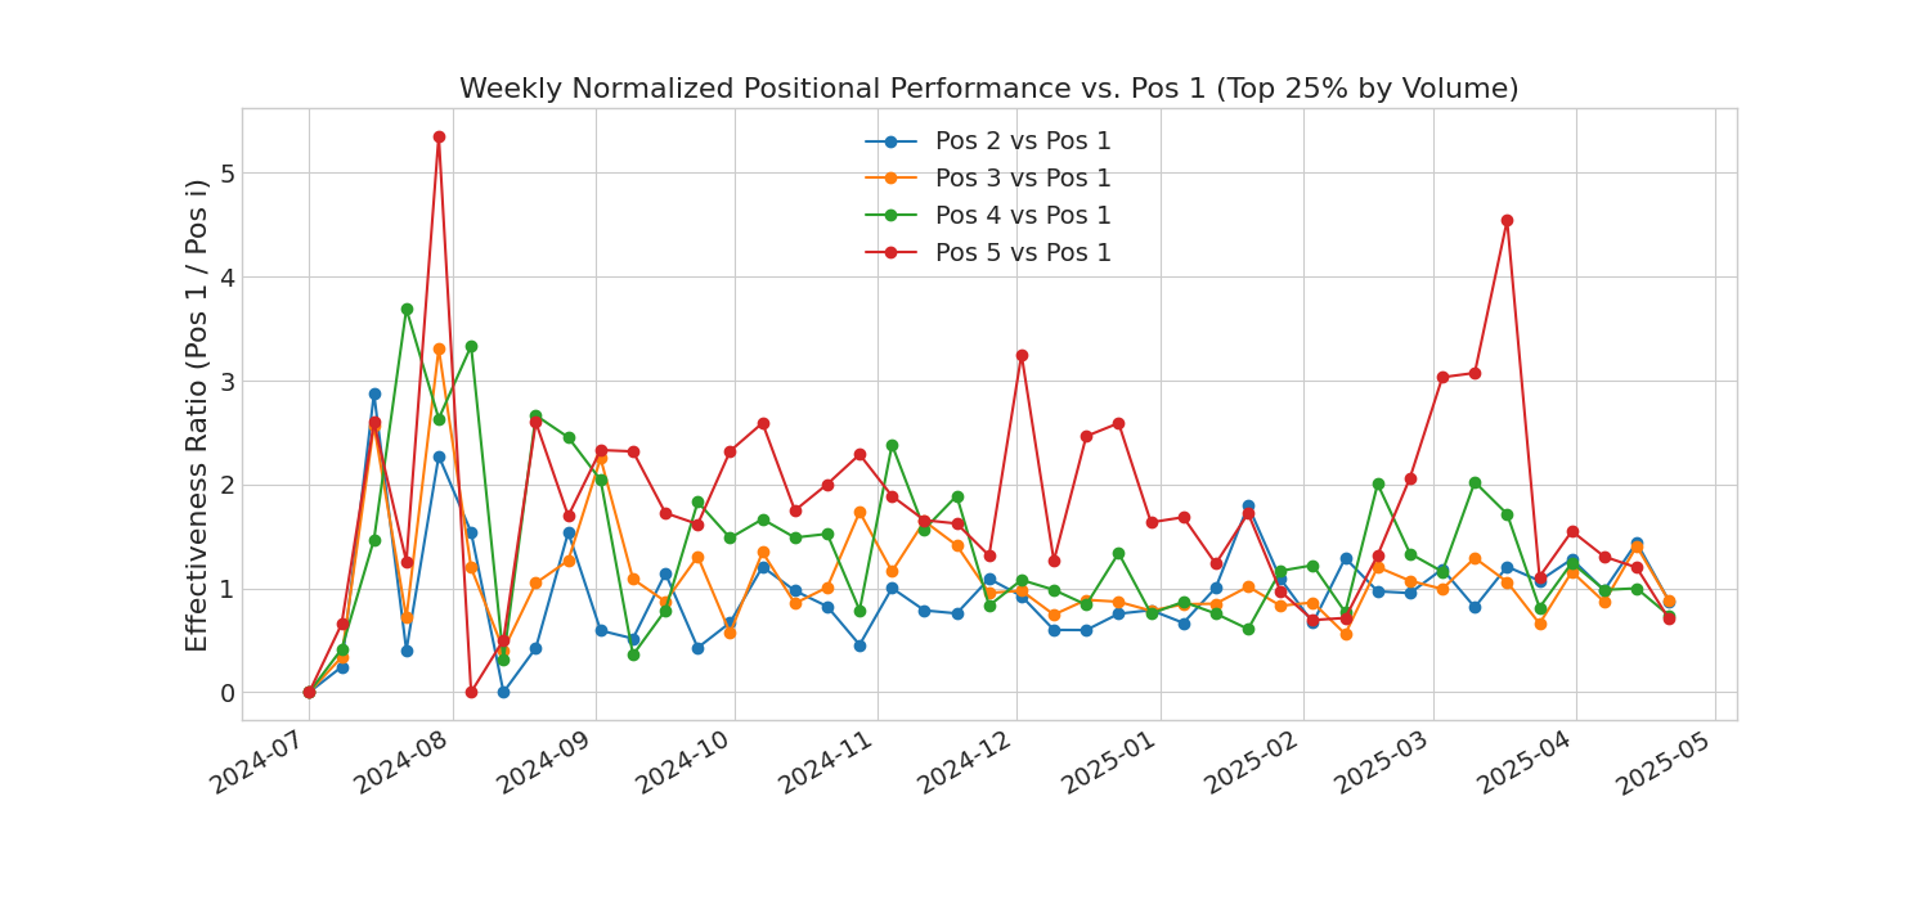
\includegraphics[width=0.85\textwidth]{figures/pos1vsothers.png}
  \caption{Effectiveness ratio of position~1 against lower positions. Ratios
           above~1, increasing with rank, quantify the advantage of the top
           slot.}
  \label{fig:pb-pos1}
\end{figure}

\paragraph{Anchored bias against external search.}
Figures~\ref{fig:pb-cg} and~\ref{fig:pb-cim} report the adjusted quality ratio
per position when the bias is anchored to Google search and to IndiaMART search
respectively, following \eqref{eq:ratio}--\eqref{eq:hist-ratios}. Both views
show the per-position ratios separating by rank and drifting upward over the
year as more history accumulates, with the lowest displayed position again the
most volatile. The two anchors give a consistent qualitative picture, which
lends confidence that the estimated bias reflects examination behaviour rather
than an artefact of any single reference source.

\begin{figure}[ht]
  \centering
  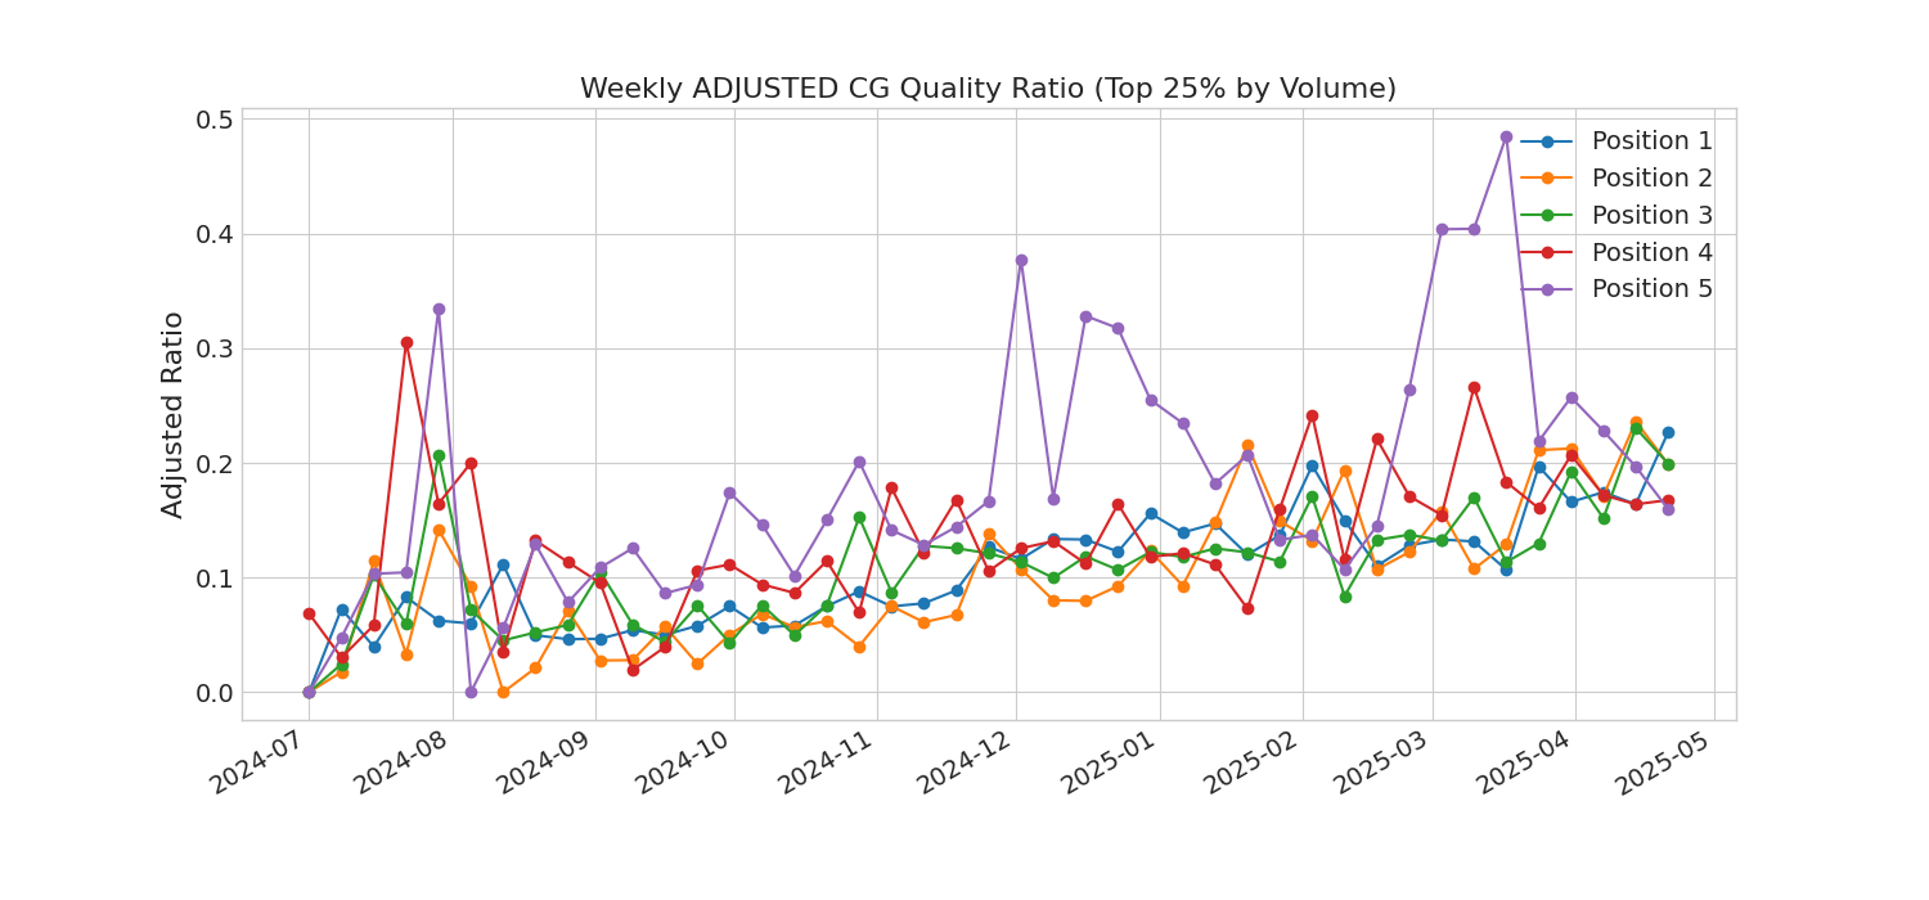
\includegraphics[width=0.85\textwidth]{figures/cg_pos.png}
  \caption{Position bias anchored to Google search. Search view counts are
           scaled to the transition view volume before forming the ratios.}
  \label{fig:pb-cg}
\end{figure}

\begin{figure}[ht]
  \centering
  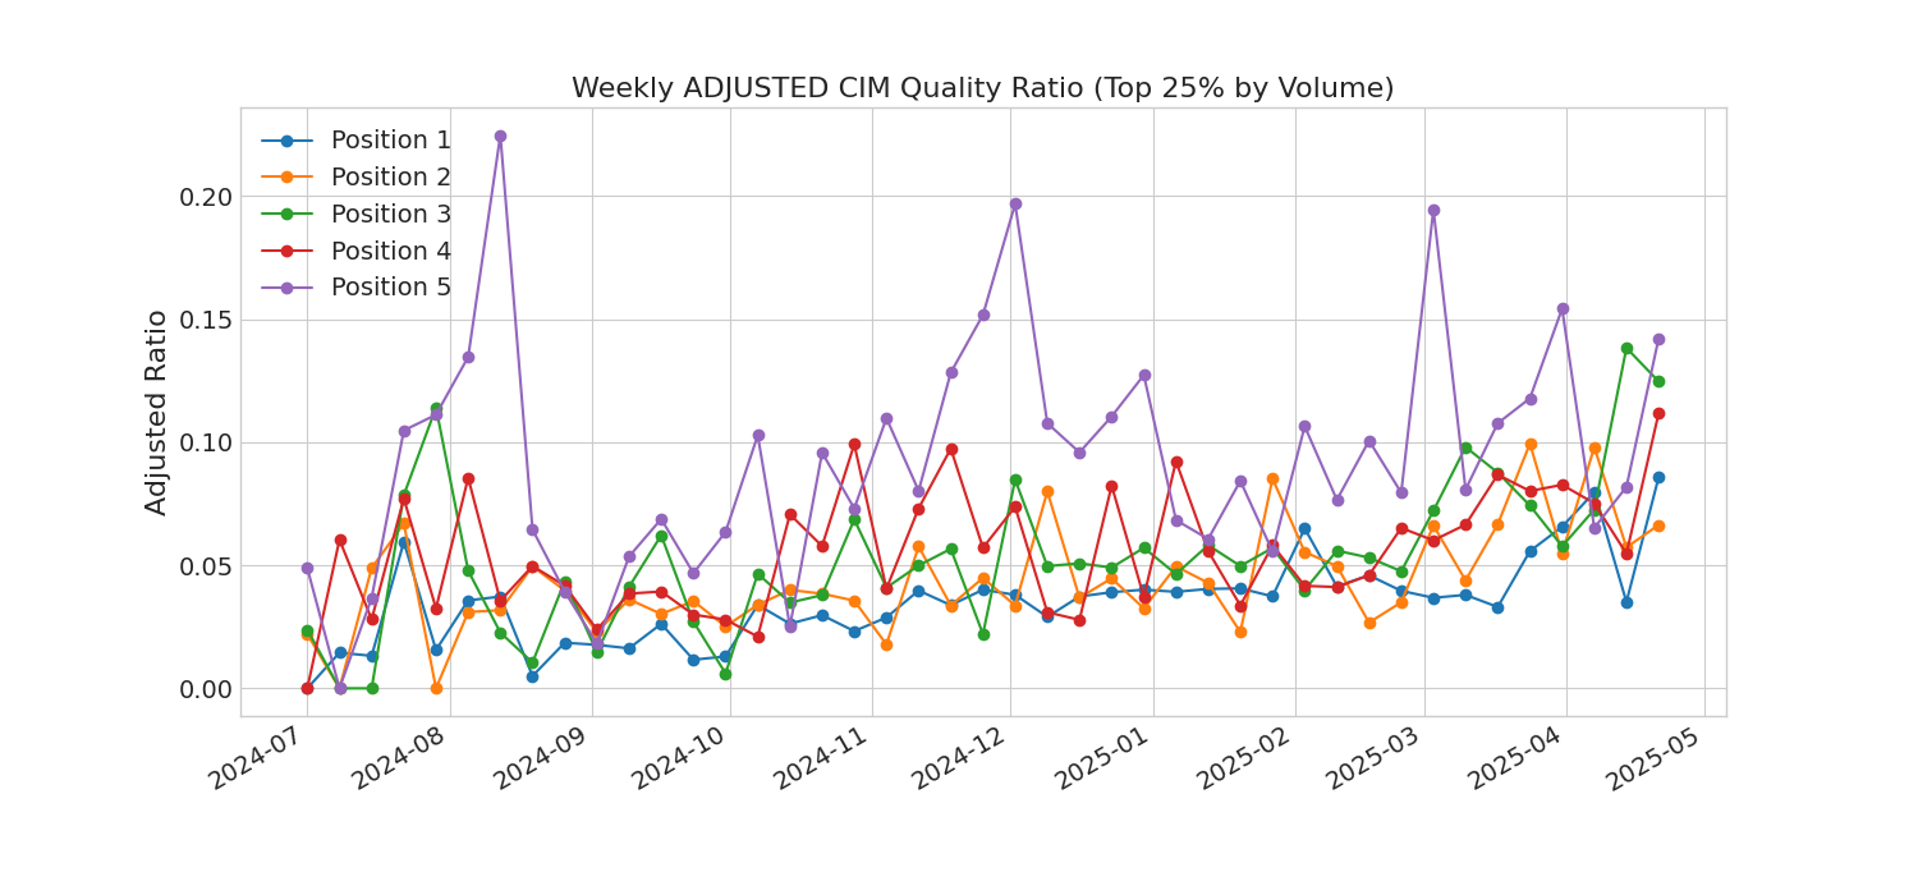
\includegraphics[width=0.85\textwidth]{figures/cim_pos.png}
  \caption{Position bias anchored to IndiaMART search, as a cross-check on the
           Google-anchored estimate of Figure~\ref{fig:pb-cg}.}
  \label{fig:pb-cim}
\end{figure}

%--------------------------------------------------------------
\section{Integration into the \texorpdfstring{$K$}{K}-Step Recommender}
\label{sec:pb-kstep}

The estimated bias is put to use inside the existing $K$-step recommendation
engine. We first sketch that engine, then describe the weighting that carries
the bias correction into it.

\subsection{The \texorpdfstring{$K$}{K}-Step Model (Background)}
\label{sec:pb-kstep-bg}
Products are treated as nodes and interactions as directed edges of a large
product-to-product graph built from session logs: an edge $i\to j$ records that
a user moved from product $i$ to product $j$. Two sources of signal are
combined. The \emph{interaction matrix} $P$ is built from weighted user
transitions; the \emph{backfill matrix} $B$ is built from precomputed offline
recommendations, in which the recommendation at rank $r$ for a product
contributes weight $1/r$. These are blended into a single transition operator
\begin{equation}
  \label{eq:blend}
  M \;=\; \alpha P + (1-\alpha)\,B,
\end{equation}
where $\alpha$ controls how far session behaviour is trusted relative to the
offline backfill. Recommendations are then generated by a $k$-step diffusion.
For a source product $s$ a one-hot vector $F^{(0)}$ places all mass on $s$, the
blended operator is applied iteratively, and the per-step distributions are
combined with a geometric decay $\lambda$:
\begin{equation}
  \label{eq:diffusion}
  F_{\text{final}} \;=\; \sum_{i=1}^{k} \lambda^{\,i-1} F^{(i)} .
\end{equation}
To keep the computation feasible at catalogue scale, each step (except the
last) is pruned to the top-$K$ neighbours per row so the matrices stay sparse;
the final score matrix is row-normalised, the top-$N$ products per row are taken
as recommendations, and an optional city-distance filter retains only products
within a given distance threshold. This engine is taken as given; the work of
this chapter is what feeds its edge weights.

\subsection{Bias-Weighted Transitions}
\label{sec:pb-weighting}
The dataset labels every interaction with a transition type (impression, click,
call, enquiry, and so on). The integration of position bias is carried out at
the level of these types: each transition type is assigned a weight chosen on
the basis of the estimated bias, and when transitions are counted to build the
interaction matrix $P$, each transition's contribution is multiplied by its
type's weight. The $K$-step model of Section~\ref{sec:pb-kstep-bg} is then run
unchanged on this re-weighted matrix. In effect, the bias correction reshapes
the edge weights of the graph so that the diffusion propagates a relevance
signal rather than a raw, exposure-distorted click signal.

\subsection{Bootstrapping Recommendations for Historical Evaluation}
\label{sec:pb-bootstrap}
Evaluating the model over the historical window is complicated by the fact that
no live recommendations existed for that period to compare against. To obtain a
reference, recommendations were \emph{assumed} on a rolling basis from the
interaction data itself: observing a transition $A\to B$ in which $B$ appears at
rank $k$ is taken to mean that $B$ was $A$'s recommendation at rank $k$, but
only when that rank was still vacant for $A$. Each such observation that fills a
previously vacant rank is counted as \emph{newly found}; an observation landing
on an already-occupied rank is counted as a \emph{mismatch}.

Figure~\ref{fig:pb-mismatch} tracks both quantities through the window. Early
on, almost every interaction fills a vacant slot (newly-found around $85\%$),
because the assumed recommendation lists are still largely empty. As the lists
saturate, the newly-found fraction falls (towards $25\%$) while the daily
mismatch fraction rises (from near zero towards $40\%$). The growing mismatch is
expected under a \emph{static} set of assumed recommendations and motivates
refreshing them periodically, a direction taken up as future work
(Chapter~\ref{ch:conclusion}).

\begin{figure}[ht]
  \centering
  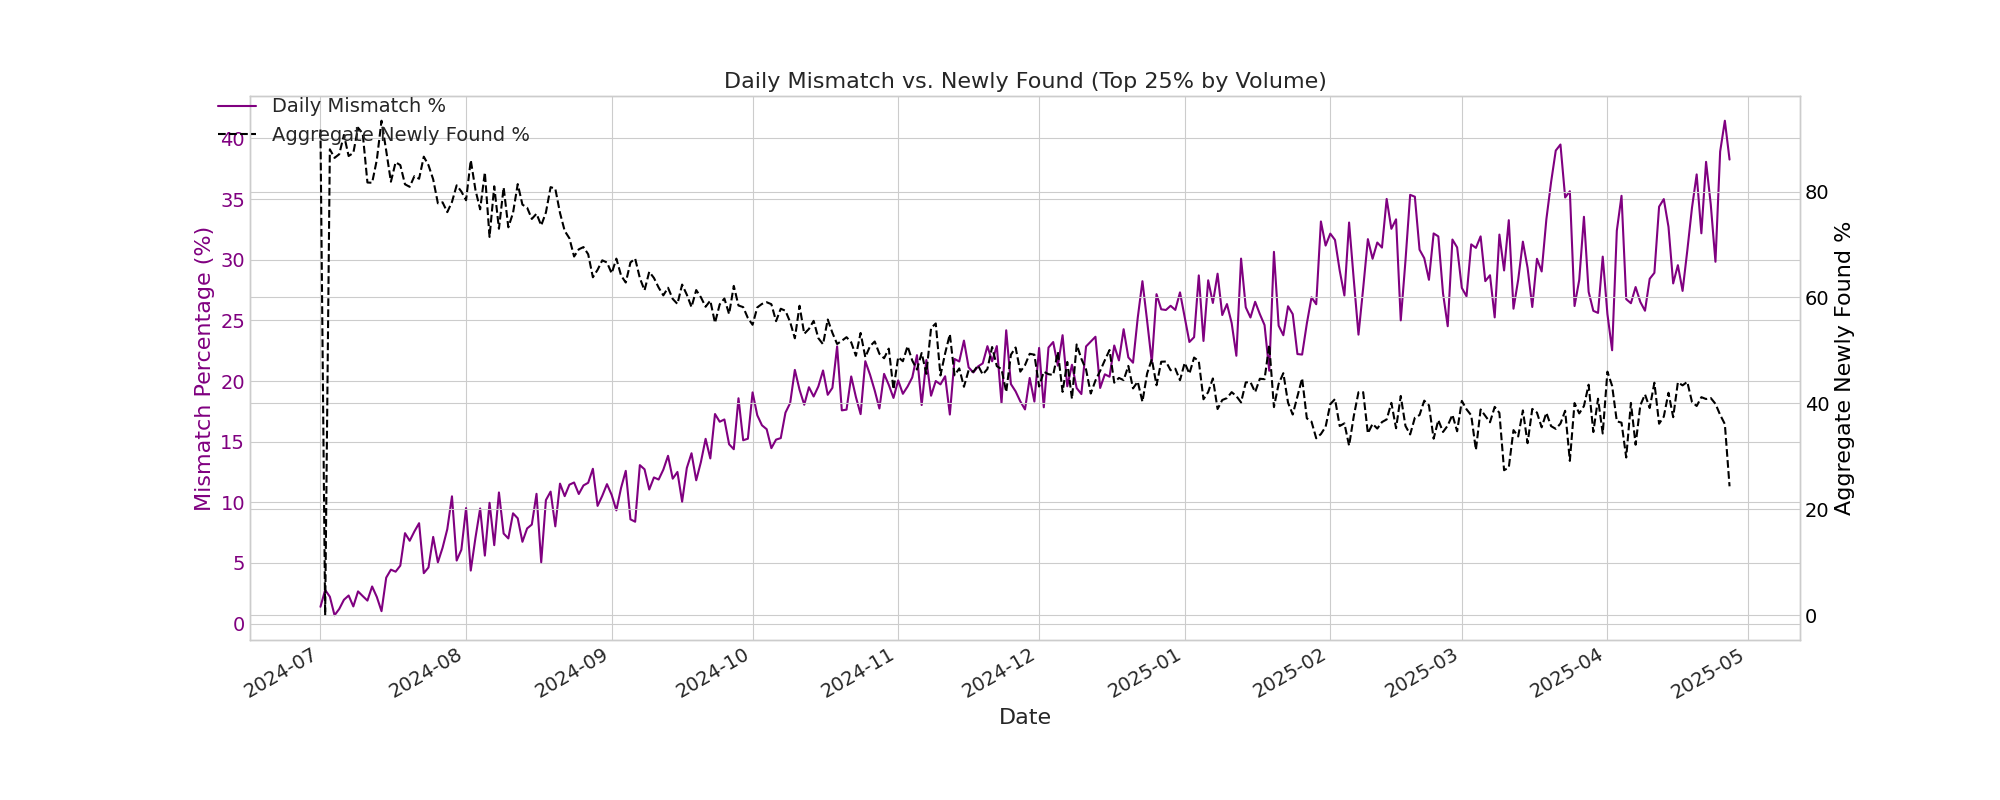
\includegraphics[width=0.9\textwidth]{figures/pb-mismatch.png}
  \caption{Bootstrapping diagnostic for the assumed recommendations. As lists
           saturate, newly-found interactions decline and mismatches grow,
           motivating periodic refresh.}
  \label{fig:pb-mismatch}
\end{figure}

%--------------------------------------------------------------
\section{Results}
\label{sec:pb-results}

The recommender was trained on the window of 1~July~2024 to 31~May~2025. At
scoring time it covered the full live catalogue of $4{,}08{,}26{,}157$ products,
generating recommendations for all of them across $684$ subcategories.
Offline evaluation measures the click-through rate (CTR) on held-out weeks of
June~2025.

Table~\ref{tab:pb-ctr} compares the unweighted $K$-step model against the
bias-weighted variant of Section~\ref{sec:pb-weighting}. Weighting the
transitions by the estimated bias raises CTR by roughly $3.5$ to $4$ percentage
points in every evaluation week --- a substantial and consistent improvement,
and direct evidence that correcting for position bias yields a better relevance
signal for the recommender.

\begin{table}[ht]
  \centering
  \caption{Offline CTR of the $K$-step recommender, unweighted versus
           bias-weighted, on held-out weeks of June~2025.}
  \label{tab:pb-ctr}
  \begin{tabular}{lccc}
    \toprule
    Evaluation week (2025) & $K$-step CTR & Bias-weighted $K$-step CTR & Gain \\
    \midrule
    01~Jun & $13.90\%$ & $17.52\%$ & $+3.62$ pp \\
    08~Jun & $13.23\%$ & $16.87\%$ & $+3.64$ pp \\
    15~Jun & $12.86\%$ & $16.55\%$ & $+3.69$ pp \\
    22~Jun & $12.32\%$ & $15.96\%$ & $+3.64$ pp \\
    \bottomrule
  \end{tabular}
\end{table}

\noindent The bias estimation of Section~\ref{sec:pb-estimate} and its
integration as transition weights thus close the loop set up at the start of the
chapter: the model is moved off the raw exposure signal and onto a
bias-corrected relevance signal, and the offline CTR improvement confirms the
correction is worthwhile.
